\chapter{Arquitectura y Diseño}\label{cap:arquitectura-diseño}

\section{Introducción}
En este capítulo, se presenta la arquitectura y el diseño del sistema implementado. Se abordan los principios y decisiones arquitectónicas que guiaron el desarrollo del sistema, así como los modelos y diagramas que ilustran la estructura y comportamiento del mismo.


\section{Modelado del sistema}
Según Somerville, el modelado de sistemas es un proceso para desarrollar modelos abstractos que representan diferentes perspectivas de un sistema. Estos modelos, que a menudo utilizan notaciones gráficas basadas en el Lenguaje de Modelado Unificado (UML), desempeñan un papel importante en la ingeniería de requerimientos y el diseño del sistema \cite{Somerville}. 
En esta sección se modelan las perspectivas de contexto o entorno, de interacción, estructural y de comportamiento para proporcionar una comprensión integral del sistema.


\subsection{Modelo de Contexto}

En la figura \ref{fig:c4-01}, se identifican dos sistemas externos que interactúan con la plataforma:

\begin{itemize}
    \item \textbf{Google Forms:} Utilizado para el envío de formularios, facilitando el ingreso de consultantes y consultas.
    \item \textbf{Email:} El sistema de correo electrónico, como Gmail, se conecta a la plataforma para el envío de notificaciones y el registro de nuevos usuarios.
\end{itemize}

Por otro lado, se encuentran los distintos tipos de usuarios que acceden a la plataforma:

\begin{itemize}
    \item \textbf{Tomadores de Caso:} Administran los casos, asignándolos a diferentes comisiones.
    \item \textbf{Jefes de Patrocinio:} Ingresan a la página de administración para gestionar permisos de usuarios, aprobar nuevos ingresos, visualizar información general y editar configuraciones.
    \item \textbf{Integrantes de Comisión:} Profesores, jefes de trabajo práctico y/o jefe de comisión que acceden al tablero de su comisión para gestionar los casos.
    \item \textbf{Alumnos:} Los alumnos no acceden directamente a la plataforma; en su lugar, envían información al profesor, quien gestiona los casos.
    \item \textbf{Clientes:} No ingresan a la plataforma; en su lugar, completan formularios que se envían al sistema.
\end{itemize}

\begin{figure}[H]
    \centering
    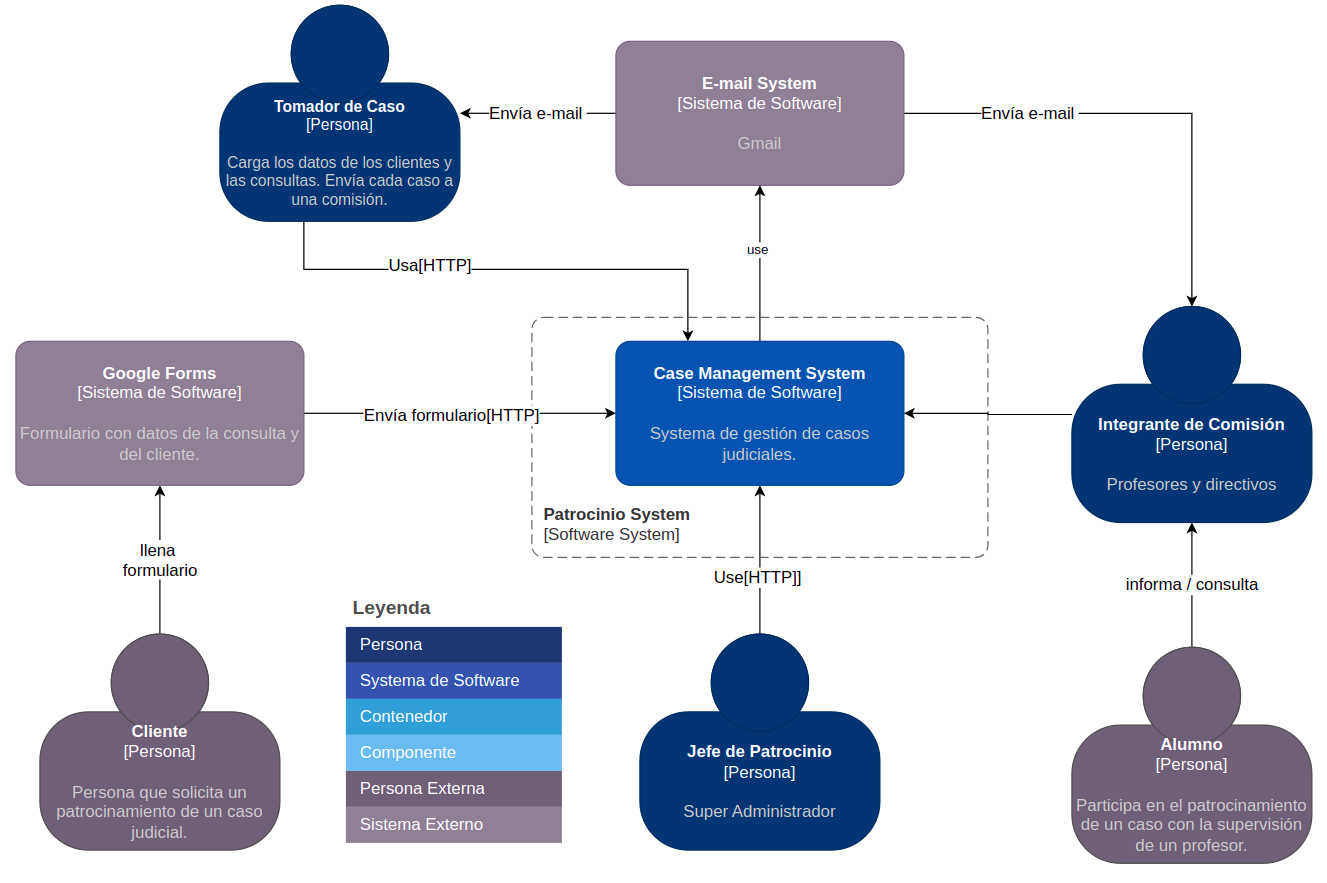
\includegraphics[width=1.1\linewidth]{fig/c4-1.png}
    \caption{Diagrama de Contexto C4}
    \label{fig:c4-01}
\end{figure}



\subsection{Modelo de Contenedores}
Si profundizamos, observamos cómo está conformado el sistema a nivel de contenedores.

Un ``contenedor'' no se limita a la noción convencional de un contenedor Docker; más bien, representa una aplicación, un almacén de datos o cualquier entidad desplegable de manera independiente, abarcando desde aplicaciones web hasta sistemas de archivos.

\begin{figure}[h]
\centering
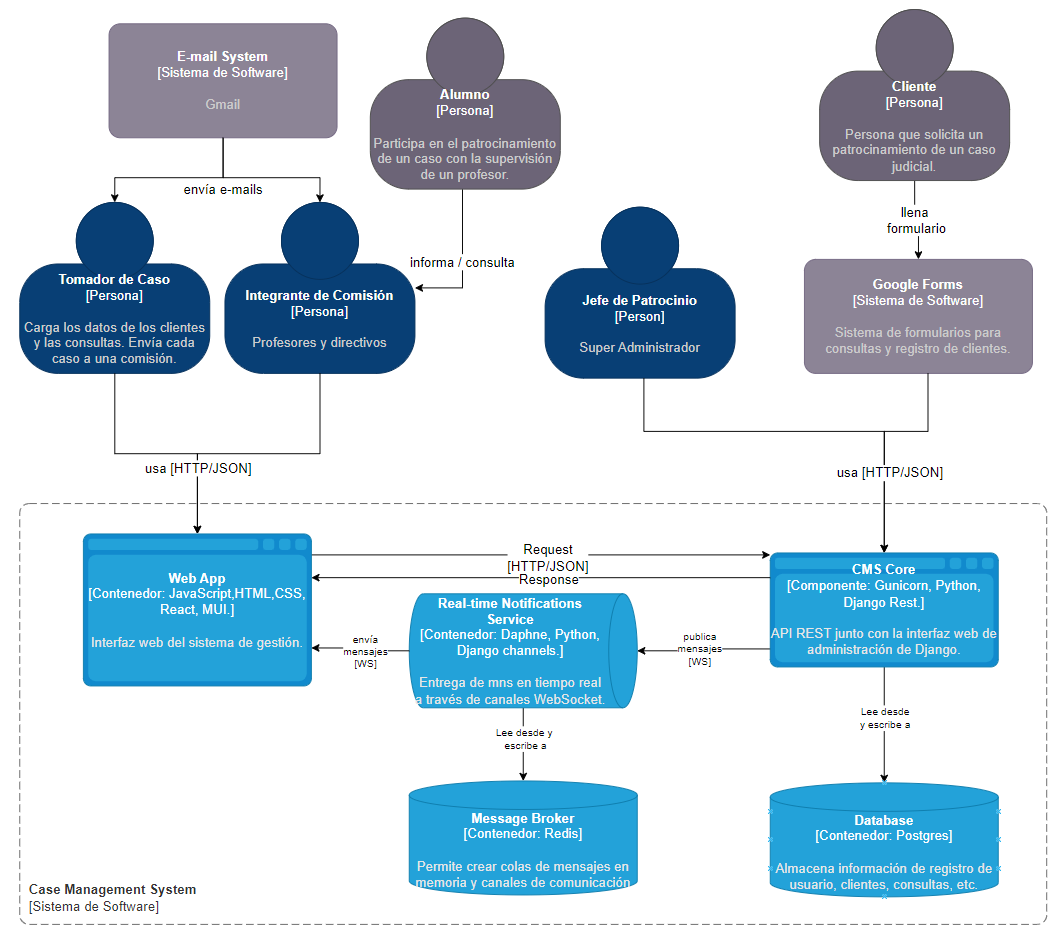
\includegraphics[width=1\linewidth]{fig/c4-2.png}
\caption{Diagrama de Contenedores C4}
\label{fig:c4-02}
\end{figure}

\begin{itemize}
\item \textbf{Web App:} Proporciona una interfaz web para el sistema de gestión de casos destinado a las comisiones y consultoría.
\item \textbf{Real-time Notifications Service:} Utiliza Django ASGI con WebSockets para la entrega de notificaciones en tiempo real.
\item \textbf{Redis:} Actúa como un almacén en memoria y se utiliza para gestionar las comunicaciones en tiempo real a través de Pub/Sub.
\item \textbf{CMS Core:} Proporciona una API REST en Django con la lógica de negocio. También ofrece la interfaz de administración de Django.
\end{itemize}




\subsection{Modelo de Componentes}
A continuación, se desglosan algunos contenedores para identificar los componentes estructurales principales y sus interacciones mediante los siguientes diagramas.

En el diagrama del contenedor CMS Core, se presentan los componentes clave y sus relaciones internas.
\begin{figure}[H]
\centering
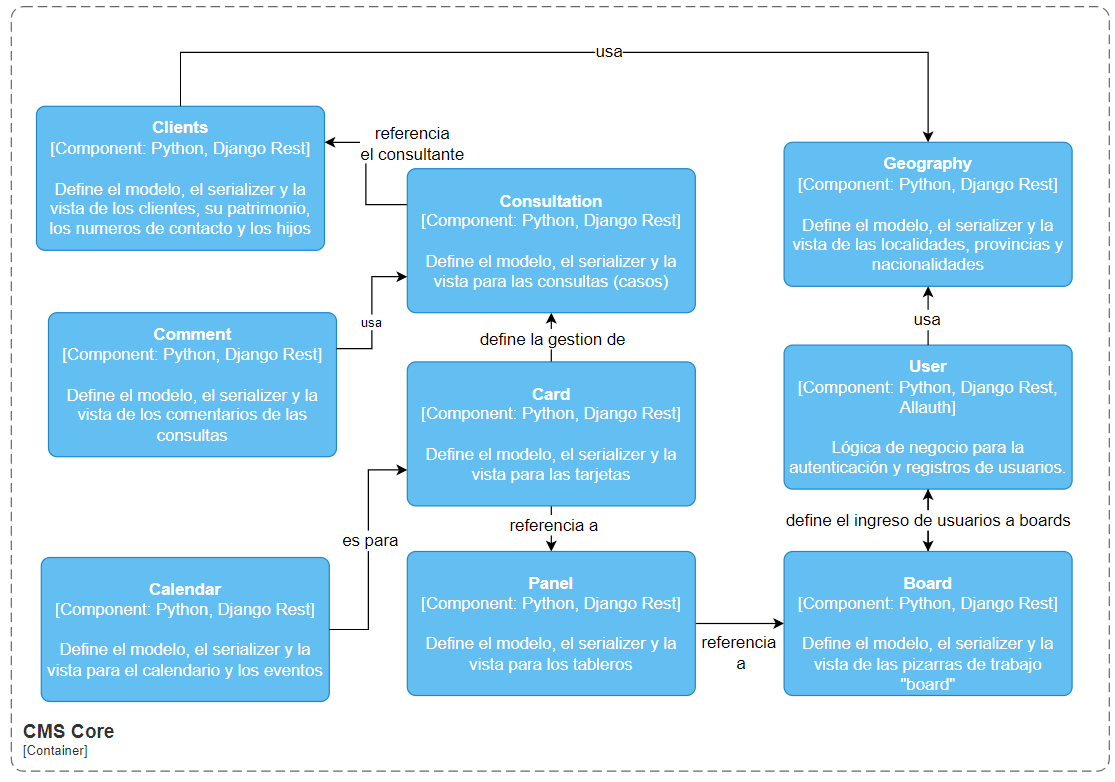
\includegraphics[width=1\linewidth]{fig/container-cms-core.png}
\caption{Diagrama de Componentes C4 del Contenedor CMS Core}
\label{fig:c4-03-cmscore}
\end{figure}
Este diagrama ilustra cómo el contenedor CMS Core incorpora cada componente de la API REST de manera modular, junto con la interfaz de usuario proporcionada por Django para la administración.

Asimismo, a continuación, se presenta el diagrama de componentes del contenedor Web App con sus principales elementos.
\begin{figure}[H]
\centering
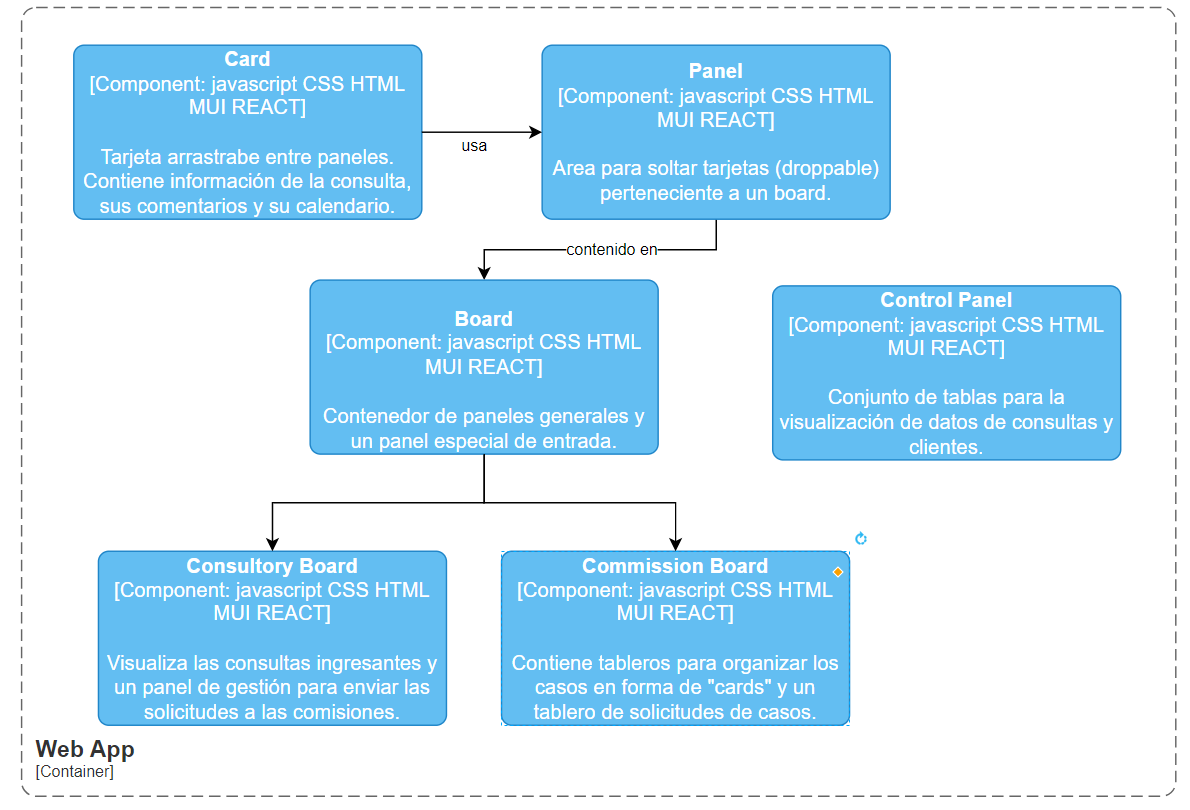
\includegraphics[width=1\linewidth]{fig/container-web-app.png}
\caption{Diagrama de Componentes C4 del Contenedor Web App}
\label{fig:c4-03-webapp}
\end{figure}
En este diagrama, se detalla la estructura del tablero (Board), que contiene paneles y, a su vez, cada panel alberga tarjetas (Cards). Además, se distinguen dos tipos de tableros: ``Consultancy'' para la consultoría y ``Commission Board'' para la pizarra de trabajo de cada comisión. Por separado, se encuentra el ``Control Panel'', que consta de dos tablas para consultas y consultantes.


\section{Arquitectura}
La implementación del software seguirá el patrón de arquitectura cliente-servidor. Esta elección se fundamenta en la necesidad de alojar la aplicación web en el servidor de aplicaciones, permitiendo a los usuarios acceder a ella desde cualquier dispositivo con conexión a internet. Se optará por la arquitectura REST para la comunicación cliente-servidor. Además, para el sistema de notificaciones, se aplicará el patrón de arquitectura Mediador (Broker Pattern), haciendo uso del diseño de publicador-suscriptor.

\section{Desarrollo Modular de la Arquitectura REST en DRF}

Cuando se menciono que la API REST está estructurada de forma modular, se refiere a que cada componente se organiza como un módulo independiente (ver \ref{section:mt-api-ref}). Cada uno de estos módulos define las rutas, modelos y vistas necesarias para su funcionamiento.

\begin{figure}[H]
\centering
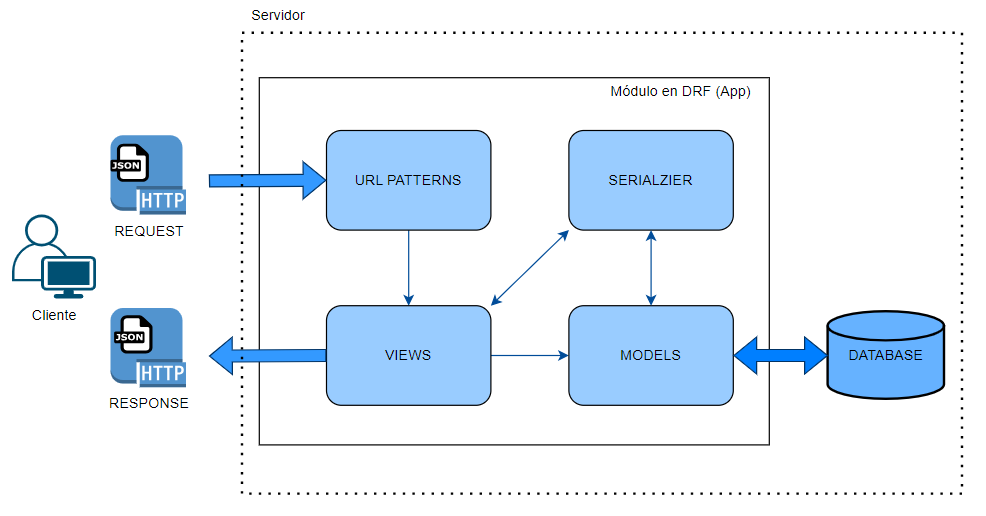
\includegraphics[width=1\linewidth]{fig/app-drf.png}
\caption{Diagrama de un Módulo en DRF}
\label{fig:app-drf}
\end{figure}

En la figura \ref{fig:app-drf}, los serializadores traducen la información de los modelos a un formato serializado (JSON) y viceversa. Las vistas establecen la lógica de negocio para manipular y procesar los datos antes de enviar una respuesta al cliente. Por otro lado, los modelos representan la estructura de los datos almacenados en la base de datos, proporcionando una abstracción entre la base de datos y las representaciones de datos expuestas a través de la API.

\section{Patrón de Arquitectura Mediador (Broker pattern)}
La implementación del patrón de arquitectura Mediador (Broker pattern) se logró mediante el uso de Django Channels y Redis como el componente Broker que coordina la comunicación entre los diversos elementos del sistema de notificaciones en tiempo real. En este contexto, el servidor publica sus servicios en el Broker, representados como ``canales'' (un canal para la consultoría y un canal por comisión).

Cuando un cliente requiere un servicio específico, se comunica con el Broker, el cual redirige al cliente hacia el servicio correspondiente según su registro.


\section{Implementación del Patrón de Diseño Pub/Sub sobre el Protocolo de comunicación Web Sockets}

En relación a la sección anterior, respecto al sistema de notificaciones en tiempor real, la implementación del patrón de diseño Publicador-Suscriptor (Pub/Sub \ref{sec:pub-sub}) sobre el protocolo de comunicación WebSockets se utiliza en la suscripción de un cliente a un canal y la publicación de mensajes del servidor a dicho canal.

\begin{figure}[H]
    \centering
    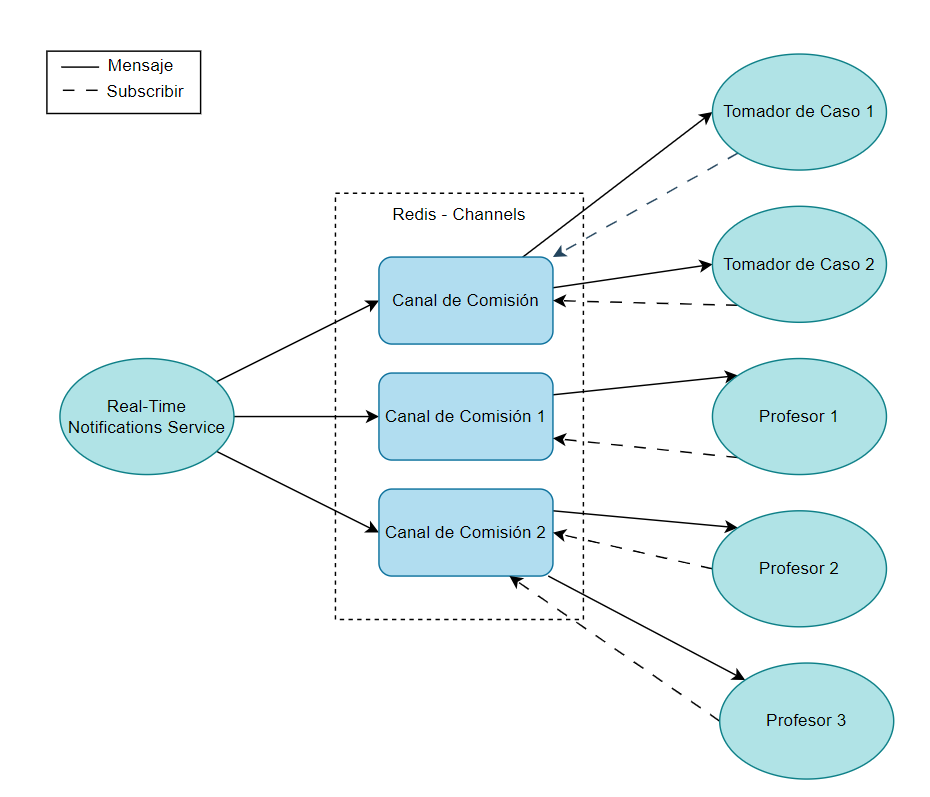
\includegraphics[width=0.9\linewidth]{fig/channels.png}
    \caption{Diagrama Implementación del Patrón Pub/Sub}
    \label{fig:channels-redis}
\end{figure}

Como se observa en la imagen, los canales representan una consultoría y un canal por cada comisión.


\section{Implementación Arrastrar y soltar}
Se utilizó el framework de JavaScript \textit{React-beautiful-dnd} para la creación de los ``Boards'', permitiendo al usuario tener una experiencia más intuitiva y rápida con la función de ``Arrastrar y soltar''. La similitud con Trello fue determinada en la etapa de gobernanza de datos y reingeniería de procesos, donde participó el equipo del Patrocinio Jurídico Gratuito de la Facultad de Derecho.

\begin{figure}[H] \centering 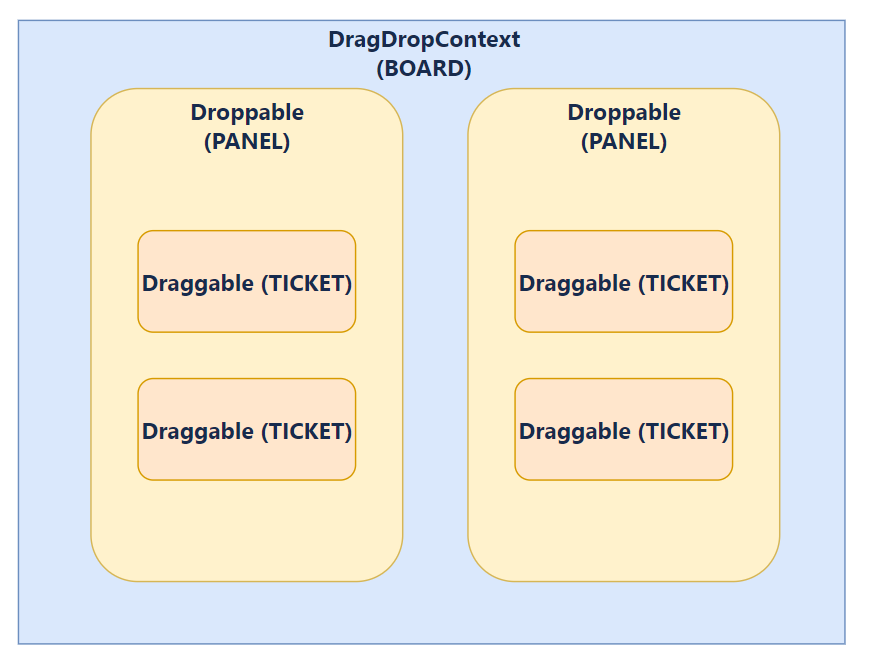
\includegraphics[width=1\linewidth]{fig/drag-drop.png} \caption{Estructura Drag and Drop} \label{fig:enter-label} \end{figure}

\begin{itemize}
    \item \textbf{DragDropContext}: Envuelve la parte de la aplicación para la que desea habilitar la función de arrastrar y soltar.
    \item \textbf{Droppable}: Esta es el área donde puede soltar y contiene.
    \item \textbf{Draggable}: Estos son los elementos que se pueden arrastrar.
\end{itemize}

A continuación, se presenta un diagrama de componentes que ilustra la estructura y relación de los elementos clave en la implementación del patrón de "Arrastrar y soltar" en el frontend.

\begin{figure}[H]
\centering
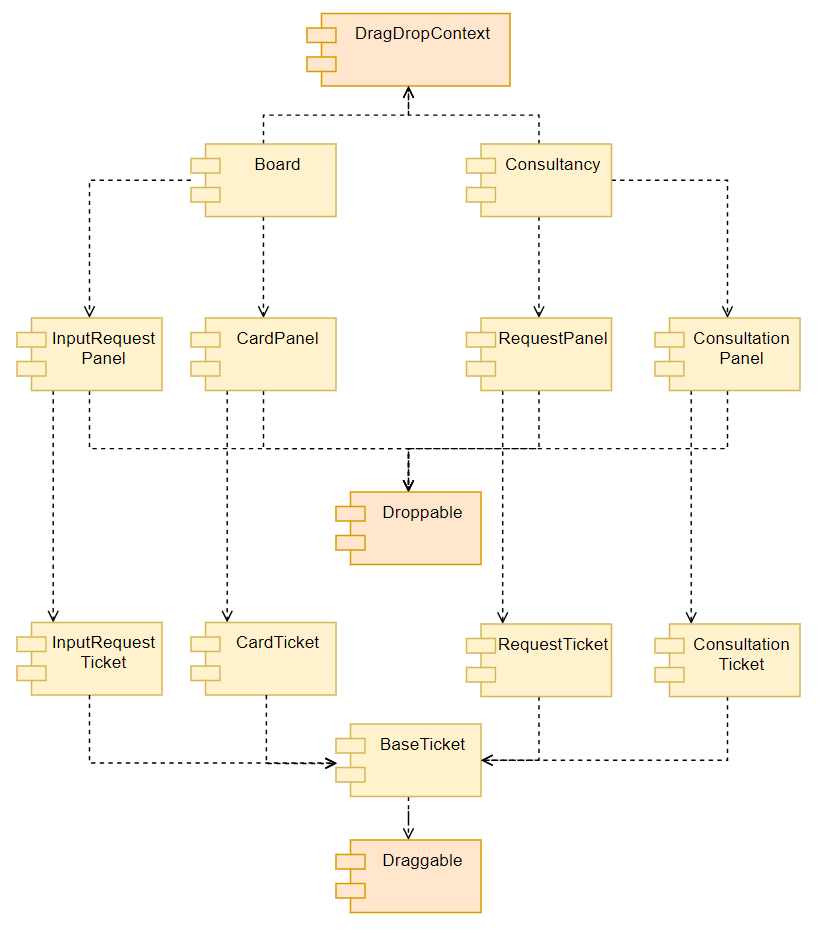
\includegraphics[width=0.90\linewidth]{fig/drag-drop-componentes.png}
\caption{Diagrama de Componentes Drag and Drop}
\label{fig:drag-drop-componentes}
\end{figure}

En la figura, se pueden observar diferentes tipos de pizarras, paneles y tickets. Cada pizarra representa un área de trabajo donde se organizan los paneles. Para cada pizarra, existen dos tipos de paneles: uno para la entrada de tickets y otro para la administración de los tickets propios de la consultoría o comisión, según corresponda. Los tickets se dividen en tres categorías: Solicitud, Consulta y Card. Los tickets de Solicitud se refieren a la solicitud de asignación de una consulta. Los tickets de Consulta son aquellos que se encuentran en la consultoría sin asignar, mientras que los tickets Card se refieren a los tickets asignados a una comisión.
